\chapter{OpenStack}
\textit{OpenStack} è una piattaforma ideata per la realizzazione e la gestione di infrastrutture cloud complesse, pubbliche e private.
Sviluppato inizialmente da \textit{NASA} e \textit{Rackspace}\footnote{Rackspace è una società che opera nell'ambito del cloud-computing con sede a Windcrest, in Texas - \textit{http://www.rackspace.com/}}, è oggi amministrato dalla \textit{OpenStack Foundation}\footnote{La \textit{OpenStack Foundation} è un'organizzazione senza scopo di lucro che promuove lo sviluppo, la distribuzione e l'adozione del progetto \textit{OpenStack}. La fondazione conta più di 18,000 membri individuali da 140 nazioni in tutto il mondo.\cite{OpenstackFoundation} \textit{https://www.openstack.org/foundation/} }, rilasciato sotto licenza Apache\footnote{La licenza Apache è una licenza di software libero, compatibile con la versione 3 della GNU GPL, non copyleft scritta dalla Apache Software Foundation (ASF). Obbliga gli utenti a preservare l'informativa di diritto d'autore e d'esclusione di responsabilità nelle versioni modificate. \textit{http://directory.fsf.org/wiki/License:Apache2.0}}, e sostenuto da aziende del calibro di \textit{IBM}, \textit{Cisco}, \textit{Citrix}, \textit{Dell}, \textit{Oracle} e \textit{Red Hat}.\cite{OpenstackWhatIs}

E' composto da una serie di progetti che si occupano dell'amministrazione delle risorse seguendo il paradigma \textit{infrastructure-as-a-service}; fornisce quindi strumenti per gestire \textit{pool} di macchine virtuali, lo \textit{storage}, e le risorse di rete all'interno di un \textit{data-center} cloud.
Il progetto è \textit{open-source} ed è interamente realizzato utilizzando il linguaggio \textit{Python}, seguendo un'architettura totalmente modulare; ogni componente è indipendente dagli altri, e può vivere anche in modalità \textit{stand-alone}.
I vari produttori solitamente producono delle derivazioni della piattaforma \textit{OpenStack}, che si differenziano tra loro per la metodologia di automazione del \textit{deployment} dei componenti e dal parco servizi offerto. Una di queste metodologie di automazione è rappresentata da \textit{DevStack} (\textit{http://docs.openstack.org/developer/devstack/}), distribuzione di \textit{OpenStack} orientata allo sviluppo e al testing.

\textit{OpenStack} è strutturato secondo un approccio \textit{multi-tenant}, ed offre un livello di astrazione tale da riuscire a garantire molte delle proprietà di sicurezza descritte nel primo capitolo.
I sorgenti sono disponibili nel repository GitHub \textit{https://github.com/openstack/}
\paragraph{}
Nell'ambito del progetto di tesi è stato utilizzato \textit{DevStack} in configurazione \textit{all-in-one}\footnote{All in one: tenendo tutti i componenti su un'unica macchina} come riferimento per implementare velocemente alcune delle proprietà di sicurezza su cui sono stati effettuati i test.
In una fase successiva è stato effettuato il \textit{deploy} manuale di un'infrastruttura più complessa distribuita su cinque nodi.

\section{Componenti di \textit{OpenStack}}
Tutti i componenti sono implementati come servizi, che espongono delle APIs \textit{REST}, invocabili tramite un'interfaccia a riga di comando o la \textit{dashboard} grafica \textit{Horizon}.
Grazie alla struttura fortemente modulare e alla natura di software \textit{open-source}, chiunque può sviluppare un proprio componente seguendo le linee guida della \textit{OpenStack Foundation}\cite{GuidelinesOpenstackHacking}.
La comunità \textit{OpenStack} ha comunque identificato una serie componenti che costituiscono il nucleo dell'intera piattaforma, essi sono considerati parte integrante del progetto e vengono perciò mantenuti ufficialmente dalla comunità stessa.
\begin{figure}[H]
\centering
\makebox[\textwidth]{
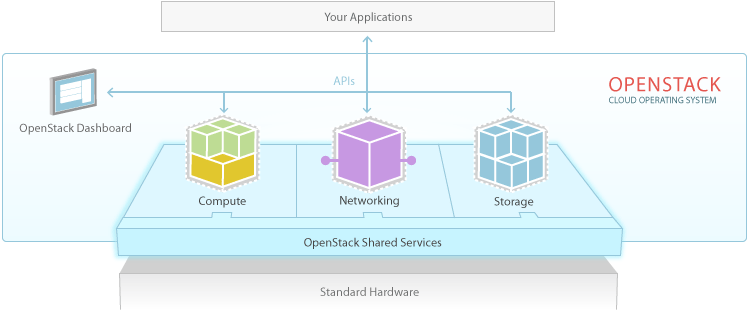
\includegraphics[width=\textwidth]{immagini/openstack-software-diagram.png}
}
\caption{Struttura della Piattaforma OpenStack\cite{OpenstackDiagram}}\label{openstacksw}
\end{figure}
\subsection{Identity service: Keystone}
\textit{Keystone} è il componente di \textit{service-catalog}, che si occupa anche di fornire i servizi di gestione delle identità, dei \textit{token} e delle politiche per l'uso specifico dei progetti nella famiglia \textit{OpenStack}.
E' l'implementazione della "\textit{Identity API}", e ha funzionalità di autenticazione basata su token (\textit{authN\footnote{AuthN: authentication}}) e meccanismi di autorizzazione di alto livello (\textit{authZ}\footnote{AuthZ: authorization}).
E' stato recentemente ristrutturato per essere espandibile e supportare meccanismi \textit{AuthN/AuthZ} come \textit{OAuth\footnote{Il framework di autorizzazione OAuth permette alle applicazioni di terze parti di ottenere l'accesso con privilegi limitati ai servizi basati su HTTP\cite{OAuth}}}, \textit{SAML\footnote{SAML, Security Assertion Markup Language, fornisce un framework basato su XML per creare e scambiare online le informazioni sulla sicurezza di un servizio tra due partner.\cite{SAML}}}, e \textit{OpenID\footnote{OpenID è un modo sicuro, veloce e facile per fornire un servizio di \textit{single-sign-on} tra siti web.\cite{OpenID}}}.
Nella pratica, si occupa di validare le credenziali degli utenti e dei servizi, rilasciare e gestire i \textit{token} di autenticazione dopo la verifica delle credenziali, e di gestire il catalogo dei servizi tenendo traccia dei relativi \textit{endpoint} e dei livelli di autorizzazione ad essi associati.
Supporta numerosi \textit{identity provider} di \textit{back-end}. L'implementazione più comune prevede l'utilizzo di MySQL per la memorizzazione dei ruoli, delle credenziali e delle sessioni, ma è possibile strutturare architetture federate tramite LDAP\footnote{Lightweight Directory Access Protocol, RFC 4510 - \textit{https://tools.ietf.org/html/rfc4510}} o meccanismi di \textit{single-sign-on}\footnote{Si parla di sistema basato su “Single Sign On” (SSO) quando le richieste di autenticazione non vengono direttamente gestite dal sistema stesso ma vengono ridirette verso un’altro sistema di autenticazione che ha precedentemente certificato le credenziali dell’utente connesso, senza quindi avere la necessità di richiedere nuovamente le credenziali per l’accesso.\cite{SSO}}.

\subsubsection{Concetti fondamentali}

\paragraph{Utente}
Rappresentazione digitale di un utente, sistema, servizio che utilizza \textit{OpenStack}.
Se è un utente ad effettuare la richiesta a \textit{Keystone} (e l'autenticazione ha esito positivo), il servizio rilascia un \textit{token} per effettuare le varie richieste.
Gli utenti hanno delle credenziali di \textit{login}, oppure dei \textit{token} per accedere alle risorse.
Possono essere direttamente assegnati ad uno o più progetti (\textit{tenant}), che costituiscono un ambiente isolato (\textit{tenant-isolation})\cite{KeystoneConcepts}
\paragraph{Credenziali}
Dati che confermano l'identità dell'utente (es: nome utente e password, nome utente e chiave API, \textit{token} di autenticazione)\cite{KeystoneConcepts}
\paragraph{Autenticazione}
Processo utilizzato per confermare l'identità di un utente, in base alle credenziali fornite.
Una volta avvenuta l'autenticazione, si procede con il rilascio di un token che verrà poi utilizzato per tutte le richieste a seguire.\cite{KeystoneConcepts}
\paragraph{\textit{Token}}
Stringa alfanumerica utilizzata per accedere alle API di \textit{OpenStack} e alle risorse. Può essere revocato in qualunque momento, ed è valido per un periodo definito.\cite{KeystoneConcepts}
\paragraph{Progetto o tenant}
Un container utilizzato per raggruppare o isolare le risorse. I tenant isolano anche gli oggetti del servizio di identità.
A seconda delle esigenze, potrebbe corrispondere a un cliente, a un'organizzazione o a un progetto.
\paragraph{Servizio}
Un servizio di \textit{OpenStack}, come \textit{Nova}, \textit{Swift}, \textit{Glance}. Un servizio è caratterizzato da uno o più \textit{endpoint}, tramite i quali gli utenti possono contattarlo per consultare le risorse da esso custodite ed eseguire le operazioni da esso consentite, nei limiti dei loro privilegi.\cite{KeystoneConcepts}
\paragraph{\textit{Endpoint}}
Un indirizzo accessibile via rete per contattare un servizio, solitamente è un URL.\cite{KeystoneConcepts}
\paragraph{Ruolo}
Una personalità con un insieme definito di privilegi e diritti, su determinate operazioni.
Il \textit{token} è legato alla lista dei ruoli dell'utente o servizio a cui si riferisce, affinché l'utente possa eseguire tutte le operazioni associate all'insieme aggregato dei ruoli a cui appartiene.\cite{KeystoneConcepts}

\begin{figure}[H]
\centering
\makebox[\textwidth]{
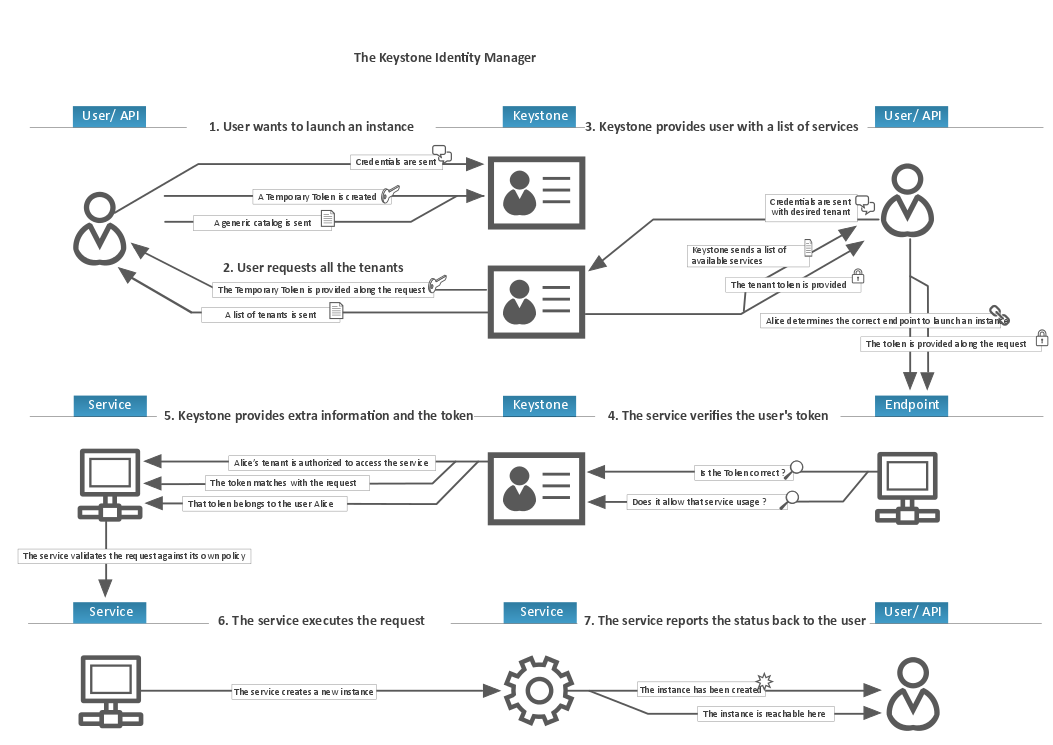
\includegraphics[width=\textwidth]{immagini/KEYSTONE.png}
}
\caption{Diagramma funzionale di Keystone\cite{KeystoneConcepts}}\label{openstackkeystone}
\end{figure}

\subsection{Compute service: Nova}
\textit{Nova} è il componente che si occupa di gestire la parte di Compute di OpenStack. La sua architettura è progettata in un'ottica di scalabilità orizzontale e poggia le sue basi sulle tecnologie di virtualizzazione note. Come hypervisor di backend, infatti, può fare uso di KVM, Xen Server, VMware ed altri.
Le sue funzionalità sono suddivise in vari servizi:
\begin{itemize}
\item \textbf{nova-api}: servizio che si occupa di gestire le richieste di allocazione e gestione delle risorse computazionali effettuate dagli utenti.
Costituisce il cuore dell'interno framework e fornisce la possibilità di controllare l'hypervisor, lo storage e le funzionalità di rete.
Gli endpoint sono servizi HTTP che gestiscono le varie funzioni utilizzando vari tipi di interfaccia (Amazon, Rackspace) e i relativi modelli. Ciò permette alle API di interagire con strumenti già esistenti creati da altri provider.
In un'architettura multi-nodo questo servizio viene installato ed eseguito sul nodo \textit{Controller}.
\item \textbf{nova-scheduler}: si occupa di effettuare lo scheduling delle operazioni invocate da nova-api. Funziona per mezzo di una coda, ed è in grado di individuare il nodo di Compute sul quale deve essere effettuato il deploy delle varie istanze virtuali. Aggiunge dunque un livello di astrazione al fine di consentire la scalabilità orizzontale. Anche questo servizio, nel caso di setup multi-nodo, viene eseguito sul nodo \textit{Controller}.
\item \textbf{Coda di messaggi}, attraverso la quale è orchestrata l'interazione tra i nodi di compute, il controller di rete, le API, lo scheduler e gli altri componenti.
I vari worker leggono cosantemente la coda in base al loro ruolo o, per esigenze specifiche, al loro hostname.
Quando arriva un task sulla coda, il worker ad esso demandato lo esegue e rimanda indietro la risposta, portando il feedback all'utente o servizio che ha generato la richiesta iniziale.
\item \textbf{nova-compute}: è un worker che interagisce con le API dell'hypervisor per creare, eliminare, modificare le varie istanze e le risorse ad esse assegnate. Questo servizio viene generalmente eseguito sullo stesso nodo dell'hypervisor.
Si occupa di:
\begin{itemize}
\item Avviare istanze
\item Terminare istanze
\item Riavviare istanze
\item Agganciare un volume a un'istanza
\item Sganciare un volume da un'istanza
\item Ottenere l'output della console
\end{itemize}
\item \textbf{nova-network}: è il controller di rete. Si occupa principalmente di amministrare le risorse di rete sui vari host. Si occupa di:
\begin{itemize}
\item Allocare indirizzi IP fissi
\item Configurare le VLAN dei vari progetti o tenant
\item Configurare la rete sui nodi di compute
\end{itemize}
Nelle release più recenti di Openstack, \textit{nova-network} è stato sostituito da un servizio dedicato: \textit{neutron}.
\item \textbf{nova-rootwrap}: consente di interagire con le API dell'hypervisor in modo sicuro, senza essere \textit{root} sulla macchina dell'hypervisor, sostituendo il comando \textit{sudo}.
\item \textbf{nova-consoleauth, nova-novncproxy, nova-xvpvncproxy}: si occupano di fornire l'accesso KVM\footnote{Keyboard, Video, Mouse} per le macchine virtuali. Solitamente, affinché ciò possa avvenire, sono utilizzati protocolli di desktop remoto come VNC, Spice, o RDP, a seconda di quanto supportato dall'hypervisor.
Il deploy di questi servizi avviene generalmente in questo modo
\begin{itemize}
\item Un processo \textit{nova-consoleauth} sul nodo controller.
\item Un processo \textit{nova-novncproxy} o \textit{nova-xvpvncproxy} sullo stesso nodo delle \textit{nova-api} (spesso nodo Controller). La differenza tra i due, è che il primo fa uso di un client basato su HTML5, mentre l'altro sfrutta la tecnologia Java. 
\end{itemize}
Le connessioni alla console, sia che siano fatte in modo diretto, sia attraverso un proxy, passano attraverso le porte TCP comprese tra 5900 e 5999. Il firewall di ogni nodo di compute deve perciò avere la seguente regola:
\begin{python}
-A INPUT -p tcp -m multiport --dports 5900:5999 -j ACCEPT
\end{python}
\end{itemize}

\begin{figure}[H]
\centering
\makebox[\textwidth]{
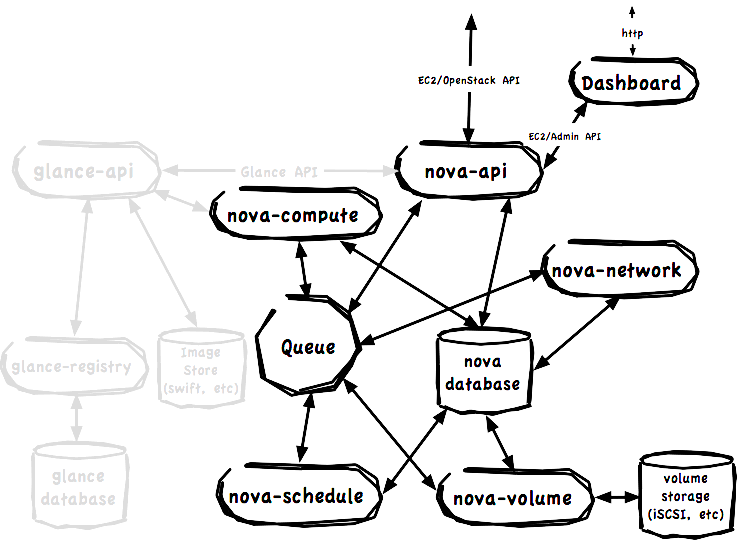
\includegraphics[width=\textwidth]{immagini/nova.png}
}
\caption{Diagramma funzionale di Nova\cite{openstacknova}}\label{openstacknova}
\end{figure}

\subsection{Image service: Glance}
\textit{Glance} si occupa della conservazione e la registrazione delle immagini di base per istanziare nuove macchine virtuali.
Il servizio espone un'interfaccia REST che consente di:
\begin{itemize}
\item reperire i metadati relativi a un'immagine
\item caricare una nuova immagine, e registrare i relativi metadati
\item scaricare un'immagine in locale
\end{itemize}
Glance fornisce la possibilità di memorizzare le immagini in varie locazioni. Esse possono infatti essere dei semplici file sul disco fisso del nodo su cui Glance è stato eseguito, oppure altri tipi di storage come Swift (il servizio di object-storage).
Esso è scritto secondo i seguenti principi:
\begin{itemize}
\item Architettura componibile
\item Alta disponibilità e scalabilità
\item Tolleranza ai guasti
\item Recuperabilità
\item Utilizzo di tecnologie standard aperte
\end{itemize}
\begin{figure}[H]
\centering
\makebox[\textwidth]{
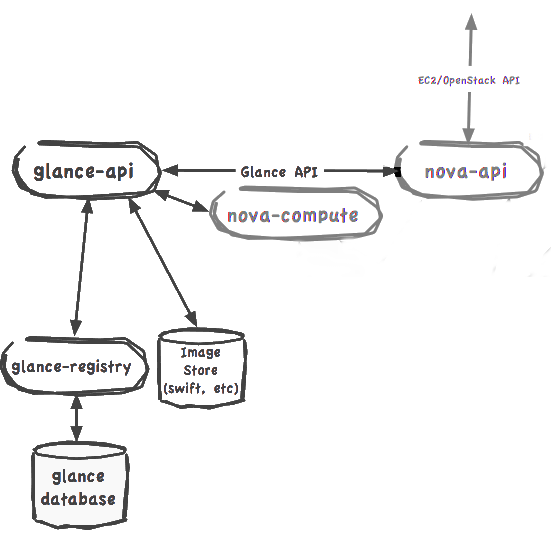
\includegraphics[scale=0.6]{immagini/glance.png}
}
\caption{Diagramma funzionale di Glance\cite{openstackglance}}\label{openstackglance}
\end{figure}


\subsection{Networking service: Neutron}
\textit{Neutron} è il componente di OpenStack che offre il servizio di "networking as a service" per le macchine virtuali, effettuando un'astrazione del livello di rete.
Lo scopo è principalmente quello di fornire delle API per strutturare la rete in modo avanzato e costruire topologie complesse, dotate di politiche di networking eterogenee.
Affinché ciò possa avvenire, Neutron fa uso di tecnologie di software-defined networking, come OpenFlow e Open-vSwitch, incapsulando il traffico con varie tecnologie di tunneling come VXLAN e GRE.
E' strutturato su un'architettura totalmente componibile tramite plug-in, che possono essere sia open-source che proprietari, i quali forniscono le modalità per amministrare in modo efficiente le capabilities di rete.
La filosofia è quindi quella di implementare l'approccio \textit{as-a-service} anche per il livello di rete, al fine di fornire le seguenti funzionalità:
\begin{itemize}
\item Load balancer-aaS
\item VPN\footnote{Virtual Private Network}-aaS
\item Firewall-aaS
\item IDS-aaS
\item etc.
\end{itemize}
Un'altra funzionalità introdotta da Neutron, è quella di creare molteplici reti virtuali e di garantire la tenancy isolation agendo direttamente sul livello 2 dello stack ISO/OSI
Le API forniscono inoltre numerosi livelli di controllo per:
\begin{itemize}
\item Politiche di sicurezza e \textit{compliance}
\item Qualità del servizio
\item Monitoraggio e risoluzione dei problemi
\end{itemize}

%http://www.slideshare.net/danwent/openstack-quantum-intro-os-meetup-32612

\begin{table}[h]
\centering
\begin{tabular}{| m{3cm}| m{5cm} | m{5cm} | }
\hline
& \textbf{Nova} & \textbf{Neutron} \\ \hline
\textit{*-as-a-service} & Compute & Network \\ \hline
\textit{Livello di astrazione} & \textbf{server virtuali}, rappresentano host con una CPU, della RAM, dischi, e interfacce di rete & \textbf{reti virtuali}: segmenti di livello 2, \textbf{porte virtuali}: punti di aggancio per i dispositivi connessi alle reti virtuali \\ \hline
\textit{Tecnologie di backend supportate} & libvirt per KVM, XenServer, Hyper-V, vMware ESX & Open vSwitch, Cisco UCS, Linux Bridge \\ \hline
\textit{Espandibilità delle API} & \textit{keypair}, ripristino delle istanze, volumi, etc. & \textit{QoS}, statistiche sulle porte, \textit{security groups}, etc. \\ \hline

\end{tabular}
\caption{Analogie tra Neutron e Nova}
\label{tab:AnalogiesNeutronNova}
\end{table}
\begin{figure}[H]
\centering
\makebox[\textwidth]{
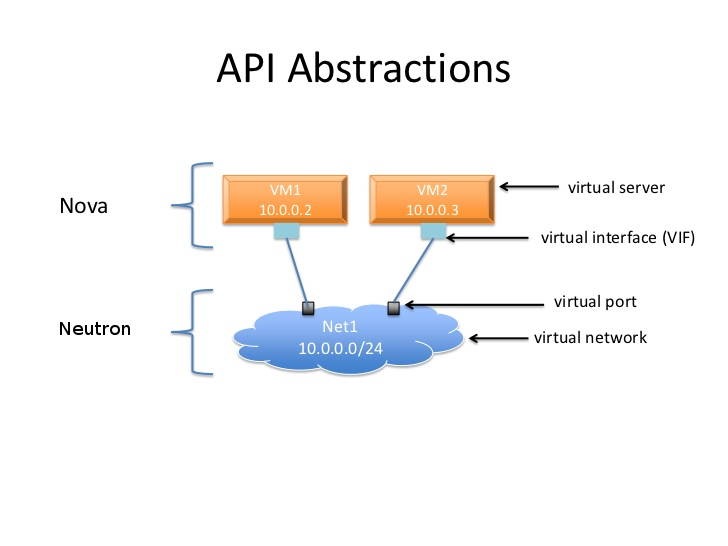
\includegraphics[width=\textwidth]{immagini/neutronNova.jpg}
}
\caption{\cite{NeutronNova}}\label{NeutronNova}
\end{figure}

\subsection{Object-storage service: Swift}
Swift è un sistema di storage di oggetti distribuito e orientato a configurazioni in alta disponibilità.
L'approccio "\textit{object-storage}" tratta i dati come oggetti binari \textit{blob} - 
Gli oggetti vengono memorizzati e referenziati generalmente tramite il protocollo HTTP, mappando in modo RESTful le azioni CRUD.
Nel caso di Swift, gli oggetti sono fisicamente memorizzati su "\textit{object-servers}".
Più "\textit{object-servers}" formano un \textit{ring}, il quale rappresenta il componente unitario per l'erogazione del servizio Swift.
Per memorizzare le informazioni relative a un oggetto, viene mantenuto un catalogo basato su metadati.
Affinché sia possibile fornire proprietà di resilienza, i \textit{rings} possono essere divisi in zone, nelle quali i dati vengono replicati in caso di guasti hardware.
Le zone possono essere rappresentate da un singolo hard disk, un server, o un dispositivo presso un datacenter esterno (che può avere ulteriori meccanismi di replica).
Per la configurazione predefinita vengono create tre repliche di ogni dato, ognuna delle quali viene memorizzata in una zona separata.
L'operazione di replica avviene in modo asincrono, ma può fallire o venire sospesa nel caso in cui il server venga spento o scollegato dall'infrastruttura, o l'infrastruttura sia sottoposta a carichi elevati.
Per questo motivo potrebbero verificarsi casi di inconsistenza dei dati.

\subsection{Block-storage service: Cinder}
\textit{Cinder} è un servizio che fornisce la possibilità di centralizzare la gestione e la creazione di volumi di storage organizzazi a blocchi.
Nello scenario più comune, i volumi Cinder rappresentano lo storage persistente alle istanze.
Permette di eseguire le operazioni di base per la gestione dei volumi di storage, di espandere i volumi, di gestirne le snapshot (i volumi sono incapsulati in file) e clonarli.
Permette inoltre di fornire un catalogo di dispositivi di storage con caratteristiche differenti (\textit{volume-types}), che possono implementare o meno determinate feature (ad es. crittografia con LUKS).
Il dispositivo di storage fisico, sia esso un disco (o un pool di dischi) magnetico o a stato solido, può essere localizzato all'interno dei server Cinder, oppure su un'architettura di storage esterna (SAN) resa disponibile ai nodi Cinder e agli hypervisors tramite canali iSCSI, NFS o Fibre Channel.
Soluzioni alternative supportate in questo senso, prevedono l'utilizzo di software come GlusterFS o RDB.

\subsection{Altri servizi}
Altri componenti di OpenStack sono
\begin{itemize}
\item{Database service: Trove}
\begin{Verbatim}[frame=single]
https://wiki.openstack.org/wiki/Trove
\end{Verbatim}
\item{Orchestration service: Heat}
\begin{Verbatim}[frame=single]
https://wiki.openstack.org/wiki/Heat
\end{Verbatim}
\item{Bare-metal provisioning service: Ironic}
\begin{Verbatim}[frame=single]
https://wiki.openstack.org/wiki/Ironic
\end{Verbatim}
\item{Data-processing service: Sahara}
\begin{Verbatim}[frame=single]
https://wiki.openstack.org/wiki/Sahara
\end{Verbatim}
\item{Messaging service: Zaqar}
\begin{Verbatim}[frame=single]
https://wiki.openstack.org/wiki/Zaqar
\end{Verbatim}
\item{Key management service: Barbican}
\begin{Verbatim}[frame=single]
https://wiki.openstack.org/wiki/Barbican
\end{Verbatim}
\item{DNS service: Designate}
\begin{Verbatim}[frame=single]
https://wiki.openstack.org/wiki/Designate
\end{Verbatim}
\item{Shared Filesystem service: Manila}
\begin{Verbatim}[frame=single]
https://wiki.openstack.org/wiki/Manila
\end{Verbatim}
\item{Application catalog service: Murano}
\begin{Verbatim}[frame=single]
https://wiki.openstack.org/wiki/Murano
\end{Verbatim}
\item{Governance service: Congress}
\begin{Verbatim}[frame=single]
https://wiki.openstack.org/wiki/Congress
\end{Verbatim}
\item{Workflow service: Mistral}
\begin{Verbatim}[frame=single]
https://wiki.openstack.org/wiki/Mistral
\end{Verbatim}
\item{Key-value store \textit{as-a-service}: MagnetoDB}
\begin{Verbatim}[frame=single]
https://wiki.openstack.org/wiki/MagnetoDB
\end{Verbatim}
\end{itemize}


\section{Servizi di supporto}
\subsection{Dashboard: Horizon}
Horizon è l'interfaccia grafica del progetto OpenStack.
Si tratta di una web-app sviluppata in Python 2.7 con framework Django, espandibile tramite vari plug-in per consentire l'integrazione con i vari componenti di OpenStack (tramite API REST).


Non è studiata nell'ottica dell'amministrazione dell'infrastruttura cloud, quanto nell'intenzione di fornire all'utente finale una dashboard per eseguire le operazioni più semplici. Per questo motivo molte funzionalità utilizzabili tramite riga di comando non sono integrate in Horizon.
Permette comunque agli amministratori di usufruire di un'interfaccia grafica di reporting sullo stato dell'infrastruttura (in termini di utilizzo della stessa, di risorse allocate e di risorse disponibili) e di effettuare operazioni ordinarie come la gestione delle utenze e dei progetti.
\begin{figure}[H]
\centering
\makebox[\textwidth]{
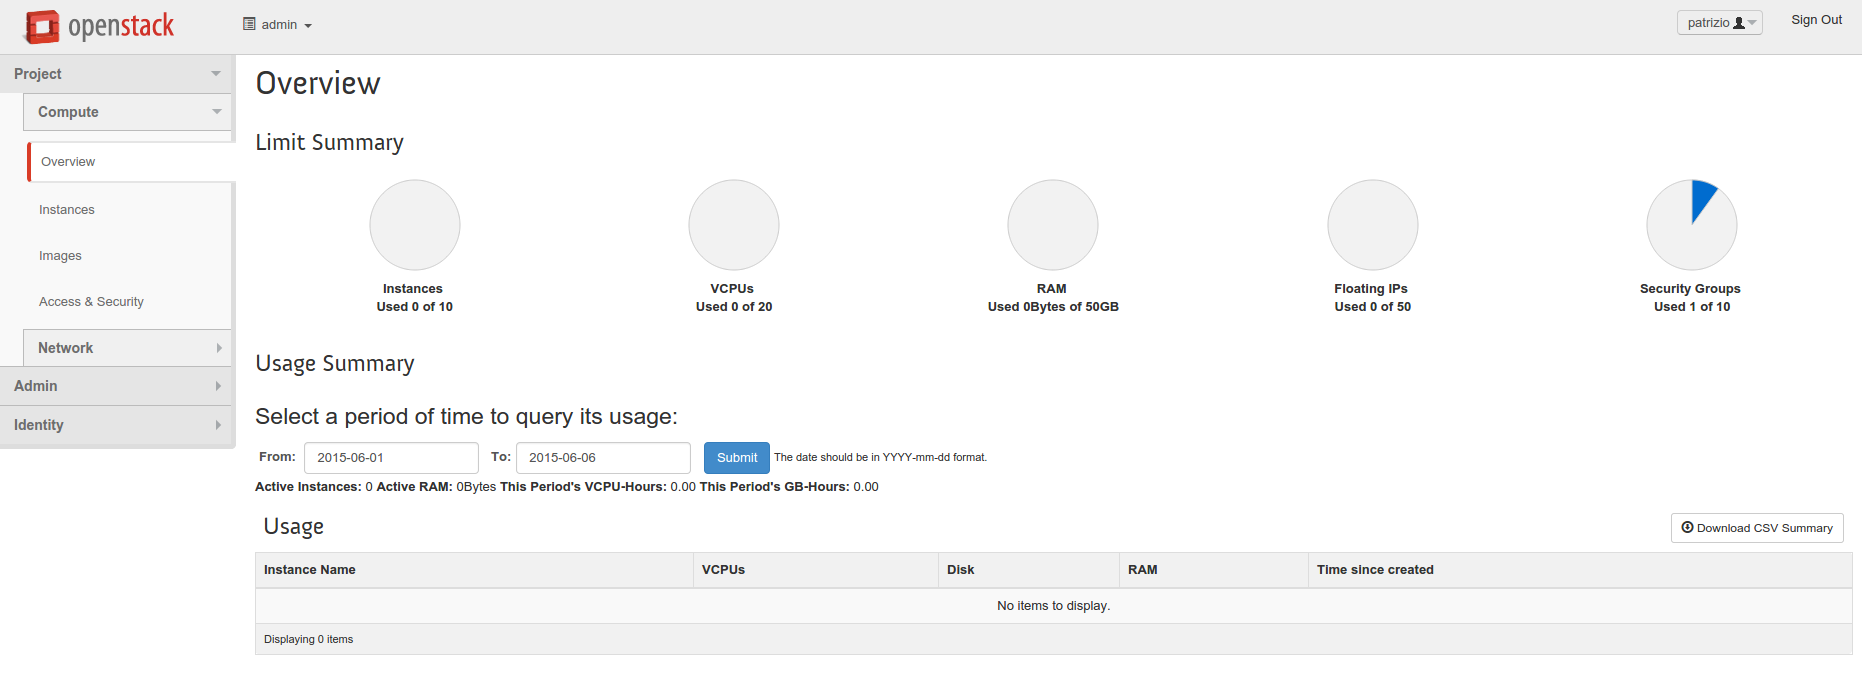
\includegraphics[width=\textwidth]{immagini/Horizon.png}
}
\caption{Horizon - Dashboard}\label{HorizonImg}
\end{figure}
\subsection{Telemetry-service: Ceilometer}
Poiché OpenStack fornisce il servizio \textit{Infrastructure-as-a-Service} ai clienti, è spesso necessario essere in grado di misurarne l'utilizzo e le performance per stabilire metriche di fatturazione, benchmarking, scalabilità e scopi statistici.
Ceilometer è il servizio di metering più promettente e maturo per l'infrastruttura OpenStack. 
Il suo nome deriva dall'ambito metereologico: il nefoipsometro (ceilometer) è infatti un dispositivo ottico, a ultrasuoni, o laser, in grado di calcolare l'altezza dello strato nuvoloso nel cielo.
Per analogia, il progetto Ceilometer costituisce un framework per il monitoraggio e la misurazione di OpenStack.
Gli obiettivi di Ceilometer sono i seguenti:
\begin{itemize}
\item Collezionamento efficiente di dati di misurazione in termini di CPU e costi di rete
\item Collezionamento dei dati provenienti dai vari servizi o da attività  di polling
\item Configurazione delle tipologie dei dati collezionati per rispettare vari requisiti operativi
\item Permettere l'accesso e l'inserimento dei dati di metering tramite APIs REST.
\item Costruzione di un framework espandibile, per collezionare anche dati provenienti da componenti \textit{ad-hoc}, tramite plugin appositamente sviluppati
\item Garantire la non repudiabilità dei dati collezionati tramite meccanismi di firma
\end{itemize}
La struttura di Ceilometer è così composta:
\begin{itemize}
\item Un'interfaccia REST per fornire l'accesso ai dati di metering contenuti nel database
\item Un agente centrale che raccoglie statistiche di utilizzo per le risorse non relative alle istanze o ai nodi di compute.
\item Agenti per i nodi di compute che raccolgono le statistiche dei nodi di compute e delle istanze.
\item Un collettore che controlla la coda dei messaggi (per le notifiche inviate dall'infrastruttura, e per i dati di misurazione provenienti dagli agenti).  I messaggi vengono poi processati, firmati, e inviati su un unico bus etichettati in modo appropriato. Il collettore può essere eseguito su uno o più server.
\item Un database per memorizzare i dati che sia in grado di gestire scritture (da parte dei collector) e letture concorrenti (da parte delle APIs REST)
\end{itemize}

Questi servizi comunicano utilizzando il bus predefinito di OpenStack. Solamente il collector e il server delle API hanno accesso al database.
I database supportati sono MongoDB, HBase, e tutti i database relazionali  supportati da SQLAlchemy.
In ogni caso in produzione è generalmente raccomandato l'utilizzo di MongoDB,  installato su un server dedicato, poiché offre meccanismi ottimizzati per l'elaborazione di letture e scritture effettuate in modo concorrente.

Le stime di utilizzo del database in un ambiente di produzione sono di 386 scritture per secondo e di circa 33 milioni di eventi al giorno, che richiedono circa 240 GB di storage al mese.

\subsection{Testing and benchmarking: Tempest e Rally}
Tempest è la test suit ufficiale di OpenStack. E' uno strumento che si occupa di eseguire un insieme di test funzionali su un'infrastruttura cluster OpenStack.
Esso esegue automaticamente vari test per ciascuna delle patch in ogni progetto di OpenStack, permettendo all'amministratore dell'infrastruttura di aggiungere funzionalità che introducano malfunzionamenti.

La complessità di Tempest è notevole, e potrebbe richiedere molto tempo per essere appreso. Inoltre manca di alcune funzionalità utili per il benchmarking, come la possibilità di effettuare simulazioni di carico e di restituire i risultati graficamente.

La soluzione a questo problema è fornita da un altro componente, Rally, che si occupa della validazione e dei test di benchmark sull'infrasatruttura OpenStack.
Rally automatizza l'installazione, la configurazione e l'esecuzione di Tempest, con la capacità di gestire automaticamente più infrastrutture.

Il motore di benchmarking è inoltre in grado di lavorare con simulazioni di carico, e di memorizzare i risultati dei test in un database, favorendo le attività di reporting.
\vfill
\newpage
\section{Deploy di OpenStack con DevStack}

\subsection{Devstack e SSL}

\section{Sicurezza e certificazione di OpenStack}
\vfill
\newpage
\section{Struttura di un ambiente multinodo di test}
Durante lo svolgimento del progetto di tesi è stato necessario realizzare un'infrastruttura OpenStack multinodo presso il laboratorio SESAR sulla quale effettuare i test sopra descritti.
La struttura dell'infrastruttura è mostrata nella Figura \ref{SesarStack}
\begin{figure}[H]
\centering
\makebox[\textwidth]{
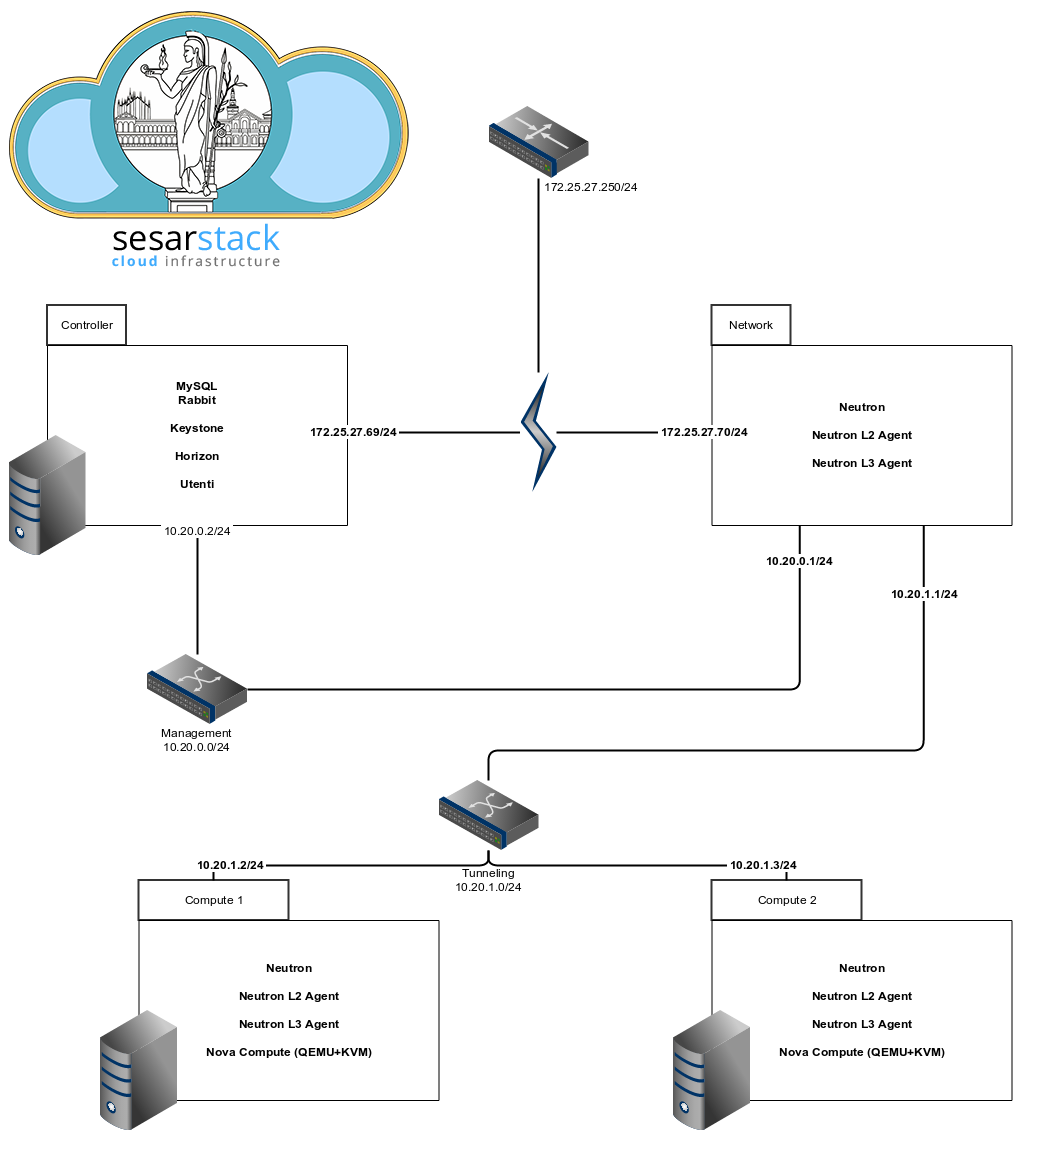
\includegraphics[width=\textwidth]{immagini/sesarstack.png}
}
\caption{Struttura Sesar Stack}\label{SesarStack}
\end{figure}